\documentclass[11pt]{article}
\usepackage{amsmath,amssymb,amsthm}
\usepackage{graphicx} \graphicspath{ {./images/} } % for images
\usepackage[margin=1in]{geometry} % for page dimensions
\usepackage{fancyhdr, enumitem, mathrsfs} % for nice headers, enumerated lists, calligraphic letters
\setlength{\parindent}{0pt}
\setlength{\parskip}{5pt plus 1pt}
\setlength{\headheight}{13.6pt}
\newcommand\question[2]{\vspace{.25in}\hrule{\textbf{#1}: #2}\vspace{.5em}\hrule\vspace{.10in}}
\renewcommand\part[1]{\vspace{.10in}\textbf{(#1)}}
\newcommand{\todo}{\fbox{TO-DO}\ \ } % for TODOs
% \newcommand\algorithm{\vspace{.10in}\textbf{Algorithm: }}
% \newcommand\correctness{\vspace{.10in}\textbf{Correctness: }}
% \newcommand\runtime{\vspace{.10in}\textbf{Running time: }}
\pagestyle{fancyplain}
\lhead{{\NAME} \\ \EMAILID}
\chead{\textbf{HW \HWNUM}}
\rhead{Capstone: Discrete Math \\ Due: December 14, 2023}
\begin{document}{\raggedright}
%Section A==============Change the values below to match your information==================
\newcommand\NAME{Ojas Chaturvedi}  % your name
\newcommand\EMAILID{oj.chaturvedi.2024@gmail.com}
\newcommand\HWNUM{10} 


\begin{question}
    {5.8.6}
    {
        Let $b_0, b_1, b_2, \ldots$ be the sequence defined by the explicit formula
        \begin{equation*}
            b_n = C \cdot 3^n + D{(-2)}^n \quad \text{for all integers $k \geq 2$}
        \end{equation*}
        where $C$ and $D$ are real numbers. Show that for any choice of $C$ and $D$,
        \begin{equation*}
            b_k = b_{k-1} + 6b_{k-2} \quad \text{for all integers $k \geq 2$}
        \end{equation*}
        \vspace{-\baselineskip}
    }
\end{question}
\begin{proof}
    {\todo}
\end{proof}

\begin{question}
    {5.8.10}
    {
        Suppose a sequence of the form $1.t.t^2.t^3 \ldots t^n \ldots$ where $t \neq 0$, satisfies the given recurrence relation (but not necessarily the initial conditions), and find all possible values of $t$.
        Suppose a sequence satisfies the given initial conditions as well as the recurrence relation, and find an explicit formula for the sequence.
        \begin{align*}
            c_k &= c_{k-1} + 6c_{k-2} & \text{for all integers $k \geq 2$} \\
            c_0 &= 0 \quad c_1=3
        \end{align*}
        \vspace{-\baselineskip}
    }
\end{question}

\begin{question}
    {5.8.15}
    {
        Suppose a sequence satisfies the given recurrence relation and initial conditions. Find an explicit formula for the sequence.
        \begin{align*}
            t_k &= 6t_{k-1} - 9t_{k-2} & \text{for all integers $k \geq 2$} \\
            t_0 &= 1 \quad t_1=3
        \end{align*}
        \vspace{-\baselineskip}
    }
\end{question}

\begin{question}
    {5.8.24}
    {
        The numbers $\frac{1 + \sqrt{5}}{2}$ and $\frac{1 - \sqrt{5}}{2}$ that appear in the explicit formula for the Fibonacci sequence are related to a quantity called the \textit{golden ration} in Greek mathematics. Consider a rectangle of length $\phi$ units and height $1$, where $\phi > 1$. \\
        \begin{figure}[h]
            \centering
            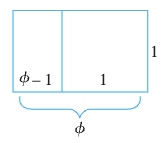
\includegraphics{5.8.24}
        \end{figure}
        \vspace{-\baselineskip}
        Divide the rectangle into a rectangle and a square as shown in the preceding diagram. The square is $1$ unit on each side, and the rectangle has sides of length $1$ and $\phi - 1$.
    }
\end{question}

\begin{question}
    {5.9.4b}
    {
        The set of arithmetic expressions over the real numbers can be defined recursively as follows:
        \vspace{-\baselineskip}
        \begin{enumerate}[label=\Roman*.]
            \item BASE:\@ Each real number $r$ is an arithmetic expression.
            \item RECURSION:\@ If $u$ and $v$ are arithmetic expressions, then the following are also arithmetic expressions:
                \begin{enumerate}
                    \item[a.] ($+u$)
                    \item[b.] ($-u$)
                    \item[c.] ($u + v$)
                    \item[d.] ($u - v$)
                    \item[e.] ($u \cdot v$)
                    \item[f.] $\left(\dfrac{u}{v} \right)$
                \end{enumerate}
            \item RESTRICTION:\@ There are no arithmetic expressions over the real numbers other than those obtained from I and II.\@
        \end{enumerate}
        \vspace{-\baselineskip}
        (Note that the \textit{expression} $\left(\dfrac{u}{v} \right)$ is legal even though the value of $v$ may be $0$.) Give derivations showing that each of the following is an arithmetic expression.
        \begin{align*}
            \left(\dfrac{(9 \cdot (6.1 + 2))}{((4-7) \cdot 6)} \right)
        \end{align*}
    }
\end{question}

\begin{question}
    {5.9.6}
    {
        Define a set $S$ recursively as follows:
        \vspace{-\baselineskip}
        \begin{enumerate}[label=\Roman*.]
            \item BASE:\@ $a \in S$
            \item RECURSION:\@ If $s \in S$, then
                \begin{enumerate}
                    \item[a.] $sa \in S$
                    \item[b.] $sb \in S$
                \end{enumerate}
            \item RESTRICTION:\@ Nothing is in $S$ other than objects defined in I and II above.
        \end{enumerate}
        \vspace{-\baselineskip}
        Use structural induction to prove that every string in $S$ begins with an $a$.
    }
\end{question}

\begin{question}
    {5.9.11}
    {
        Define a set $S$ recursively as follows:
        \vspace{-\baselineskip}
        \begin{enumerate}[label=\Roman*.]
            \item BASE:\@ $0 \in S$
            \item RECURSION:\@ If $s \in S$, then
                \begin{enumerate}
                    \item[a.] $s + 3 \in S$
                    \item[b.] $s - 3 \in S$
                \end{enumerate}
            \item RESTRICTION:\@ Nothing is in $S$ other than objects defined in I and II above.
        \end{enumerate}
        \vspace{-\baselineskip}
        Use structural induction to prove that every integer in $S$ is divisible by $3$.
    }
\end{question}

\begin{question}
    {5.9.16}
    {
        Give a recursive definition for the set of all strings of $0$'s and $1$'s for which all the $0$'s precede all the $1$'s.
    }
\end{question}

\begin{question}
    {5.9.18}
    {
        Give a recursive definition for the set of all strings of $a$'s and $b$'s that contain exactly one $a$.
    }
\end{question}

\begin{question}
    {6.1.6}
    {
        Let $A=\{x \in \mathbf{Z} \mid x=5 a+2$ for some integer $a\}$, $B=\{y \in \mathbf{Z} \mid y=10 b-3$ for some integer $b\}$, and $C=\{z \in \mathbf{Z} \mid z=10 c+7$ for some integer $c\}$. Prove or disprove each of the following statements.
        \vspace{-\baselineskip}
        \begin{enumerate}
            \item[a.] $A \subseteq B$
            \item[b.] $B \subseteq A$
            \item[c.] $B=C$
        \end{enumerate}
    }
\end{question}

\begin{question}
    {6.1.20}
    {
        Let $B_i=\{x \in \mathbf{R} \mid 0 \leq x \leq i\}$ for all integers $i=1,2,3,4$.
        \vspace{-\baselineskip}
        \begin{enumerate}
            \item[a.] $B_1 \cup B_2 \cup B_3 \cup B_4=$ ?
            \item[b.] $B_1 \cap B_2 \cap B_3 \cap B_4=$ ?
            \item[c.] Are $B_1, B_2, B_3$, and $B_4$ mutually disjoint? Explain.
        \end{enumerate}
    }
\end{question}

\begin{question}
    {6.1.23}
    {
        Let $V_i=\left\{x \in \mathbf{R} \mid-\dfrac{1}{i} \leq x \leq \dfrac{1}{i}\right\}=\left[-\dfrac{1}{i}, \dfrac{1}{i}\right]$ for all positive integers $i$.
        \vspace{-\baselineskip}
        \begin{enumerate}
            \item[a.] $\bigcup_{i=1}^4 V_i=$ ?
            \item[b.] $\bigcap_{i=1}^4 V_i=$ ?
            \item[c.] Are $V_1, V_2, V_3, \ldots$ mutually disjoint? Explain.
            \item[d.] $\bigcup_{i=1}^n V_i=$ ?
            \item[e.] $\bigcap_{i=1}^n V_i=$ ?
            \item[f.] $\bigcup_{i=1}^{\infty} V_i=$ ?
            \item[g.] $\bigcap_{i=1}^{\infty} V_i=$ ?
        \end{enumerate}
    }
\end{question}

\begin{question}
    {6.1.33}
    {
        \vspace{-\baselineskip}
        \begin{enumerate}
            \item[a.] Find $\mathscr{P}(\emptyset)$.
            \item[b.] Find $\mathscr{P}(\mathscr{P}(\emptyset))$.
            \item[c.] Find $\mathscr{P}(\mathscr{P}(\mathscr{P}(\emptyset)))$.
        \end{enumerate}
    }
\end{question}

\begin{question}
    {6.2.10}
    {
        Use an element argument to prove the statement.
        Assume that all sets are subsets of a universal set $U$.
        For all sets $A, B$, and $C$,
        \begin{align*}
            (A-B) \cap(C-B)=(A \cap C)-B \text{. }
        \end{align*}
        \vspace{-\baselineskip}
    }
\end{question}

\begin{question}
    {6.2.14}
    {
        Use an element argument to prove the statement.
        Assume that all sets are subsets of a universal set $U$.
        For all sets $A, B$, and $C$, if $A \subseteq B$ then $A \cup C \subseteq B \cup C$.
    }
\end{question}

\begin{question}
    {6.2.32}
    {
        Use the element method for proving a set equals the empty set to prove the statement.
        Assume that all sets are subsets of a universal set $U$.
        For all sets $A, B$, and $C$, if $A \subseteq B$ and $B \cap C=\emptyset$ then $A \cap C=\emptyset$.
    }
\end{question}

\begin{question}
    {6.2.39}
    {
        Prove the statement.
        For all integers $n \geq 1$, if $A_1, A_2, A_3, \ldots$ and $B$ are any sets, then
        \begin{align*}
            \bigcap_{i=1}^n (A_i - B) = \left(\bigcap_{i=1}^n A_i \right) - B \text{. }
        \end{align*}
    }
\end{question}

\end{document}